% called by main.tex
%
\renewcommand{\chaptername}{Part}
\chapter{Distributions, Estimations and Confidence Interval}
\label{part1}
In this section, we will visually represent the distribution of global GDP per capita and life expectancy. Subsequently, we will undertake the estimation of key statistical parameters, specifically the \textit{mean} value and \textit{standard deviation}. Furthermore, an analysis will be conducted to establish the 95\% confidence interval for the mean value within each respective field.
\section{Distributions \& estimations}
As stated in many textbooks, the sample mean $\overline{x}$ can be used to estimate the population mean $\mu$.
\begin{center}
    {\fontsize{16}{20}\selectfont $\overline{x} = \frac{1}{n} \sum_{i = 1}^{n} x_i$}
\end{center}

And the unbiased standard deviation is approximated using this formula:
\begin{center}
{\fontsize{16}{20}\selectfont$s = \sqrt{\frac{1}{n-1}\sum_{i=1}^n (x_i - \overline{x})^2} $}
\end{center}

Excel offers the \textit{AVG} and \textit{STDEV} functions for the computation of the mean and standard deviation, thereby facilitating a straightforward approach to data analysis.

Additionally, we provided a Jupyter notebook file containing our analytical findings for visualization. Leveraging libraries such as \href{https://pandas.pydata.org/}{pandas} and \href{https://numpy.org/}{NumPy}, computations can be streamlined further. The employment of \textit{mean} and \textit{std} functions from NumPy serves to efficiently calculate these statistical values.

The following is the code in Python used for calculating these values.
\newpage
\begin{verbatim}
    gdp = df['GDP'].to_numpy()
    lex = (pd.to_numeric(df['LEX'].str.replace(',', '.'), errors='coerce'))\
        .to_numpy()
    size = gdp.size
    gdp_mean = np.mean(gdp)
    lex_mean = np.mean(lex)
    gdp_sd = np.std(gdp)
    lex_sd = np.std(lex)
    print("Observations: ", size)
    print("GDP(mean, standard deviation): ", gdp_mean, gdp_sd)
    print("LEX(mean, standard deviation): ", lex_mean, lex_sd)
\end{verbatim}

Result:
\begin{verbatim}
    Observations:  195
    GDP(mean, standard deviation):  20872.102564102563 24179.09720483299
    LEX(mean, standard deviation):  72.39435897435897 7.319704279746025
\end{verbatim}


Furthermore, we have visualized the data through the creation of a histogram, enhancing accessibility and comprehension of the dataset's distribution.
\begin{figure}[hbpt]
    \centering
    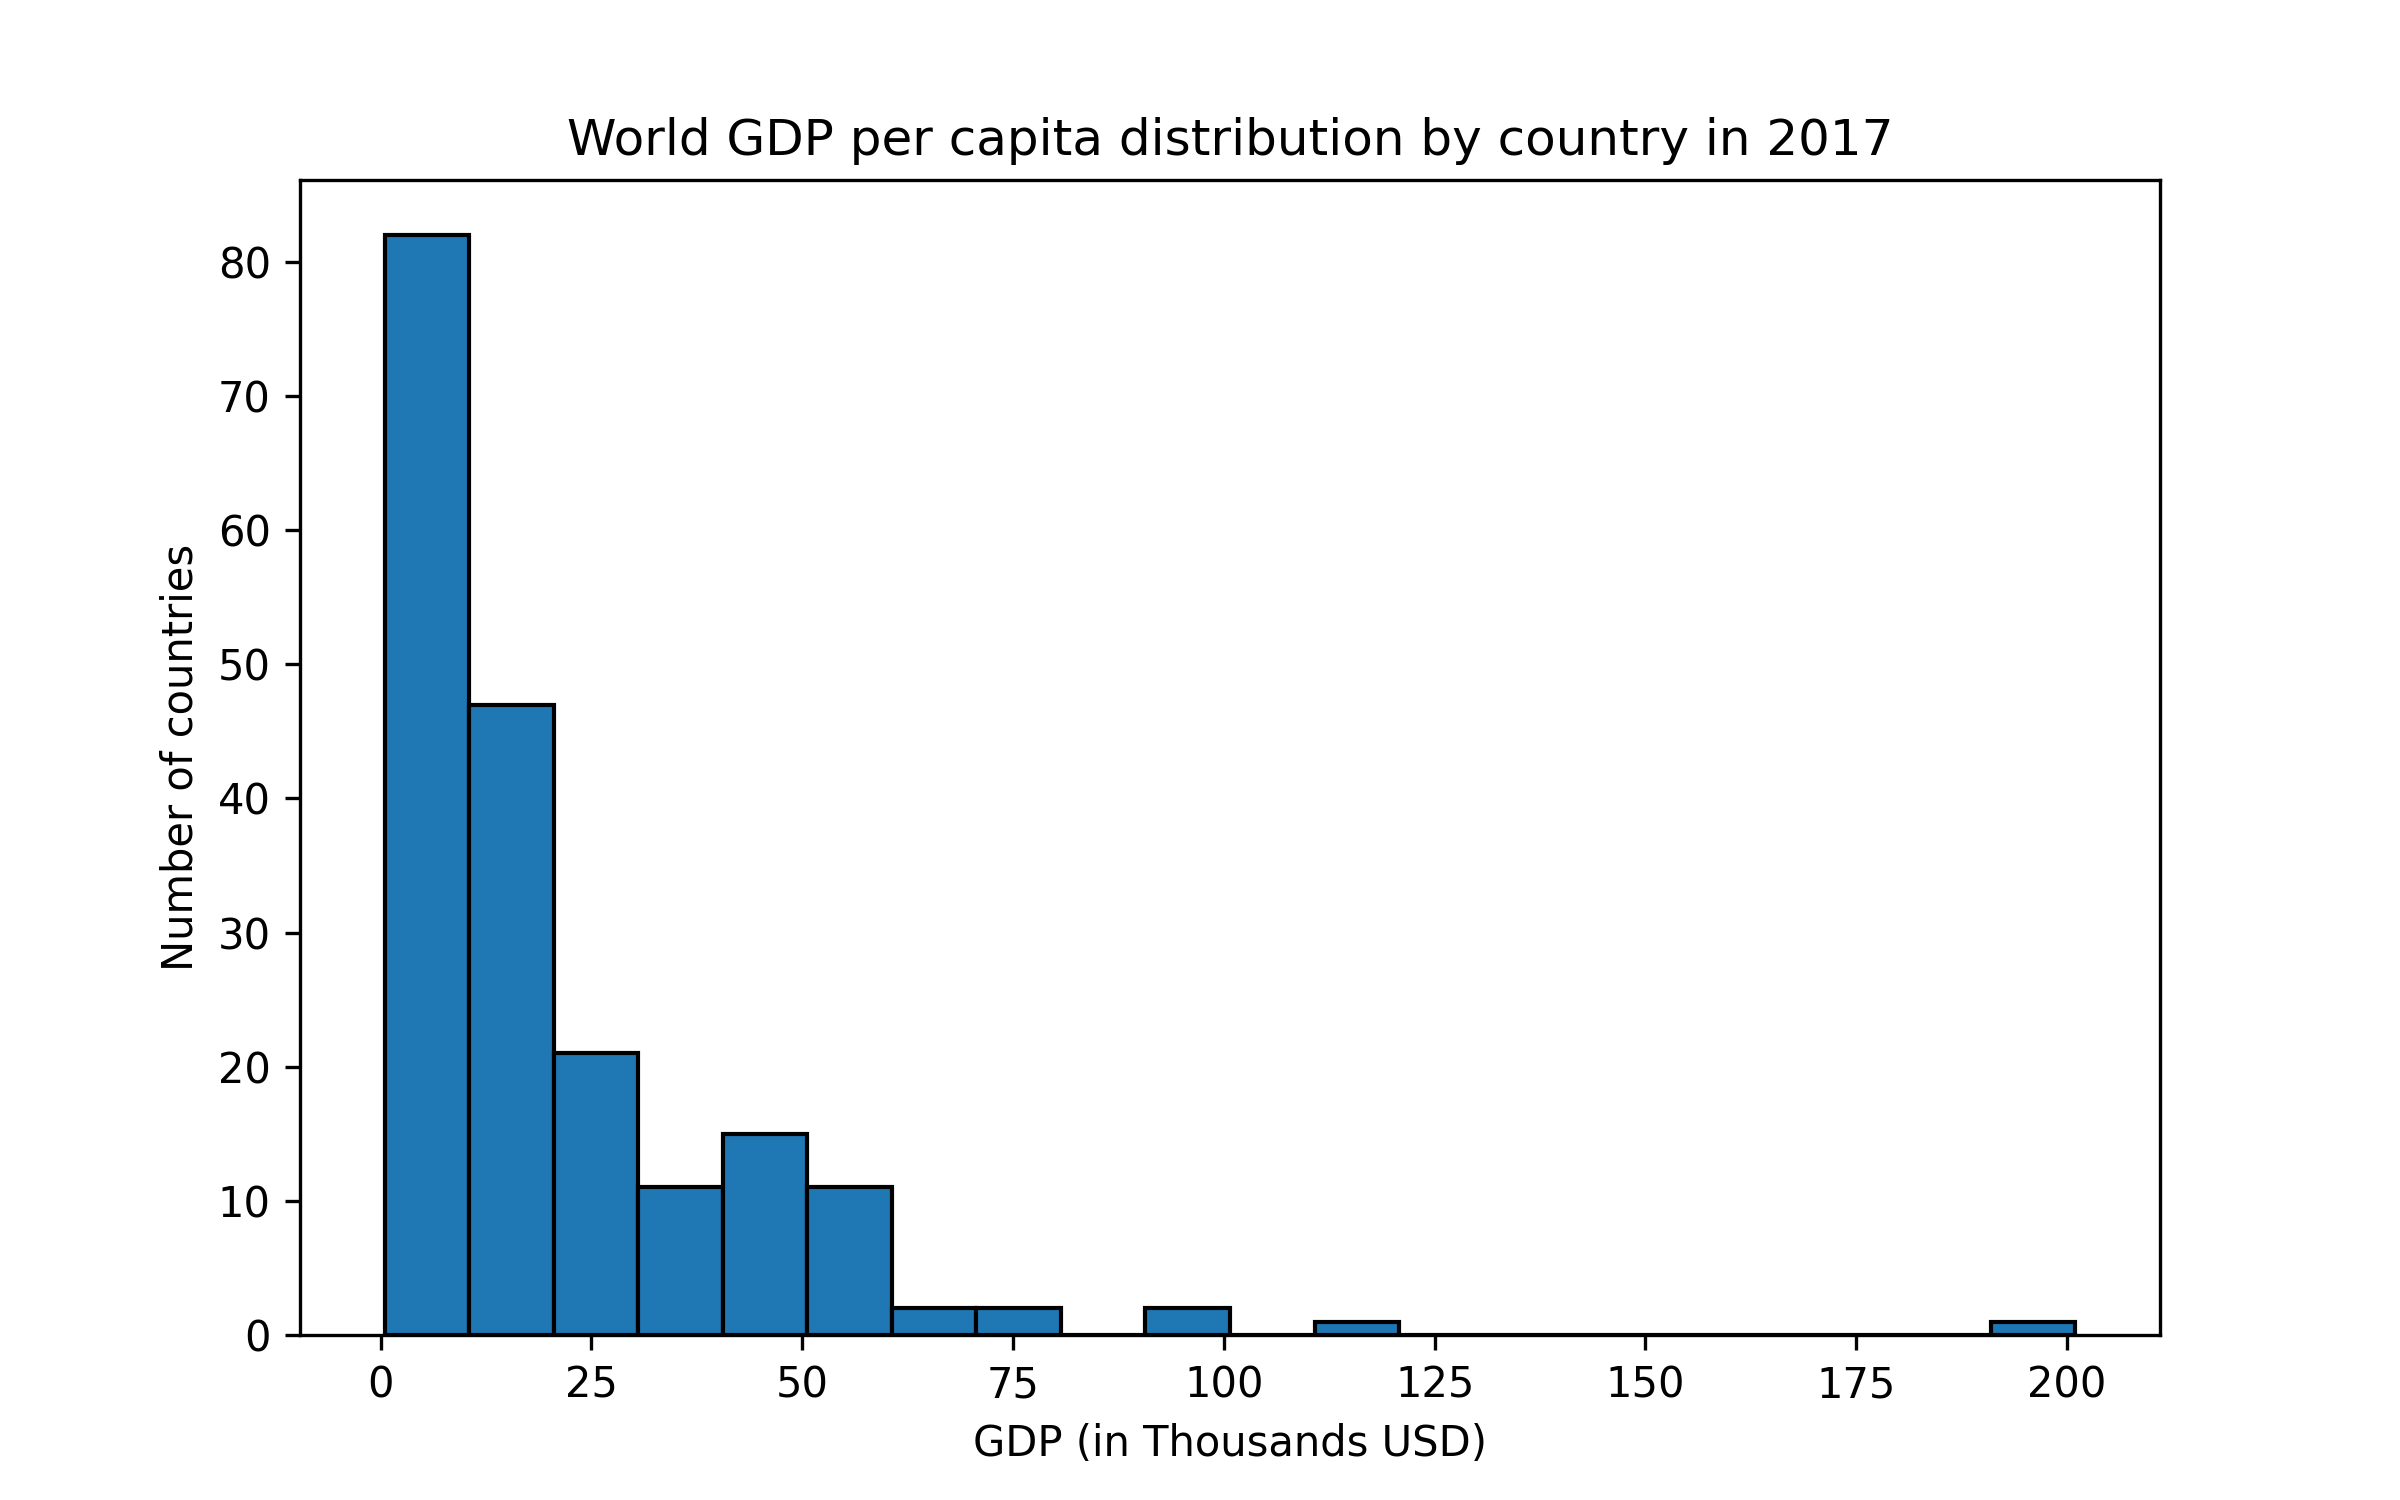
\includegraphics[width=0.8\textwidth]{figures/gdp_histo.png}
    \caption{Distribution of GDP per capita in 2017}
    \label{fig:gdp-dis}
\end{figure}
\newpage
\begin{figure}[t]
    \centering
    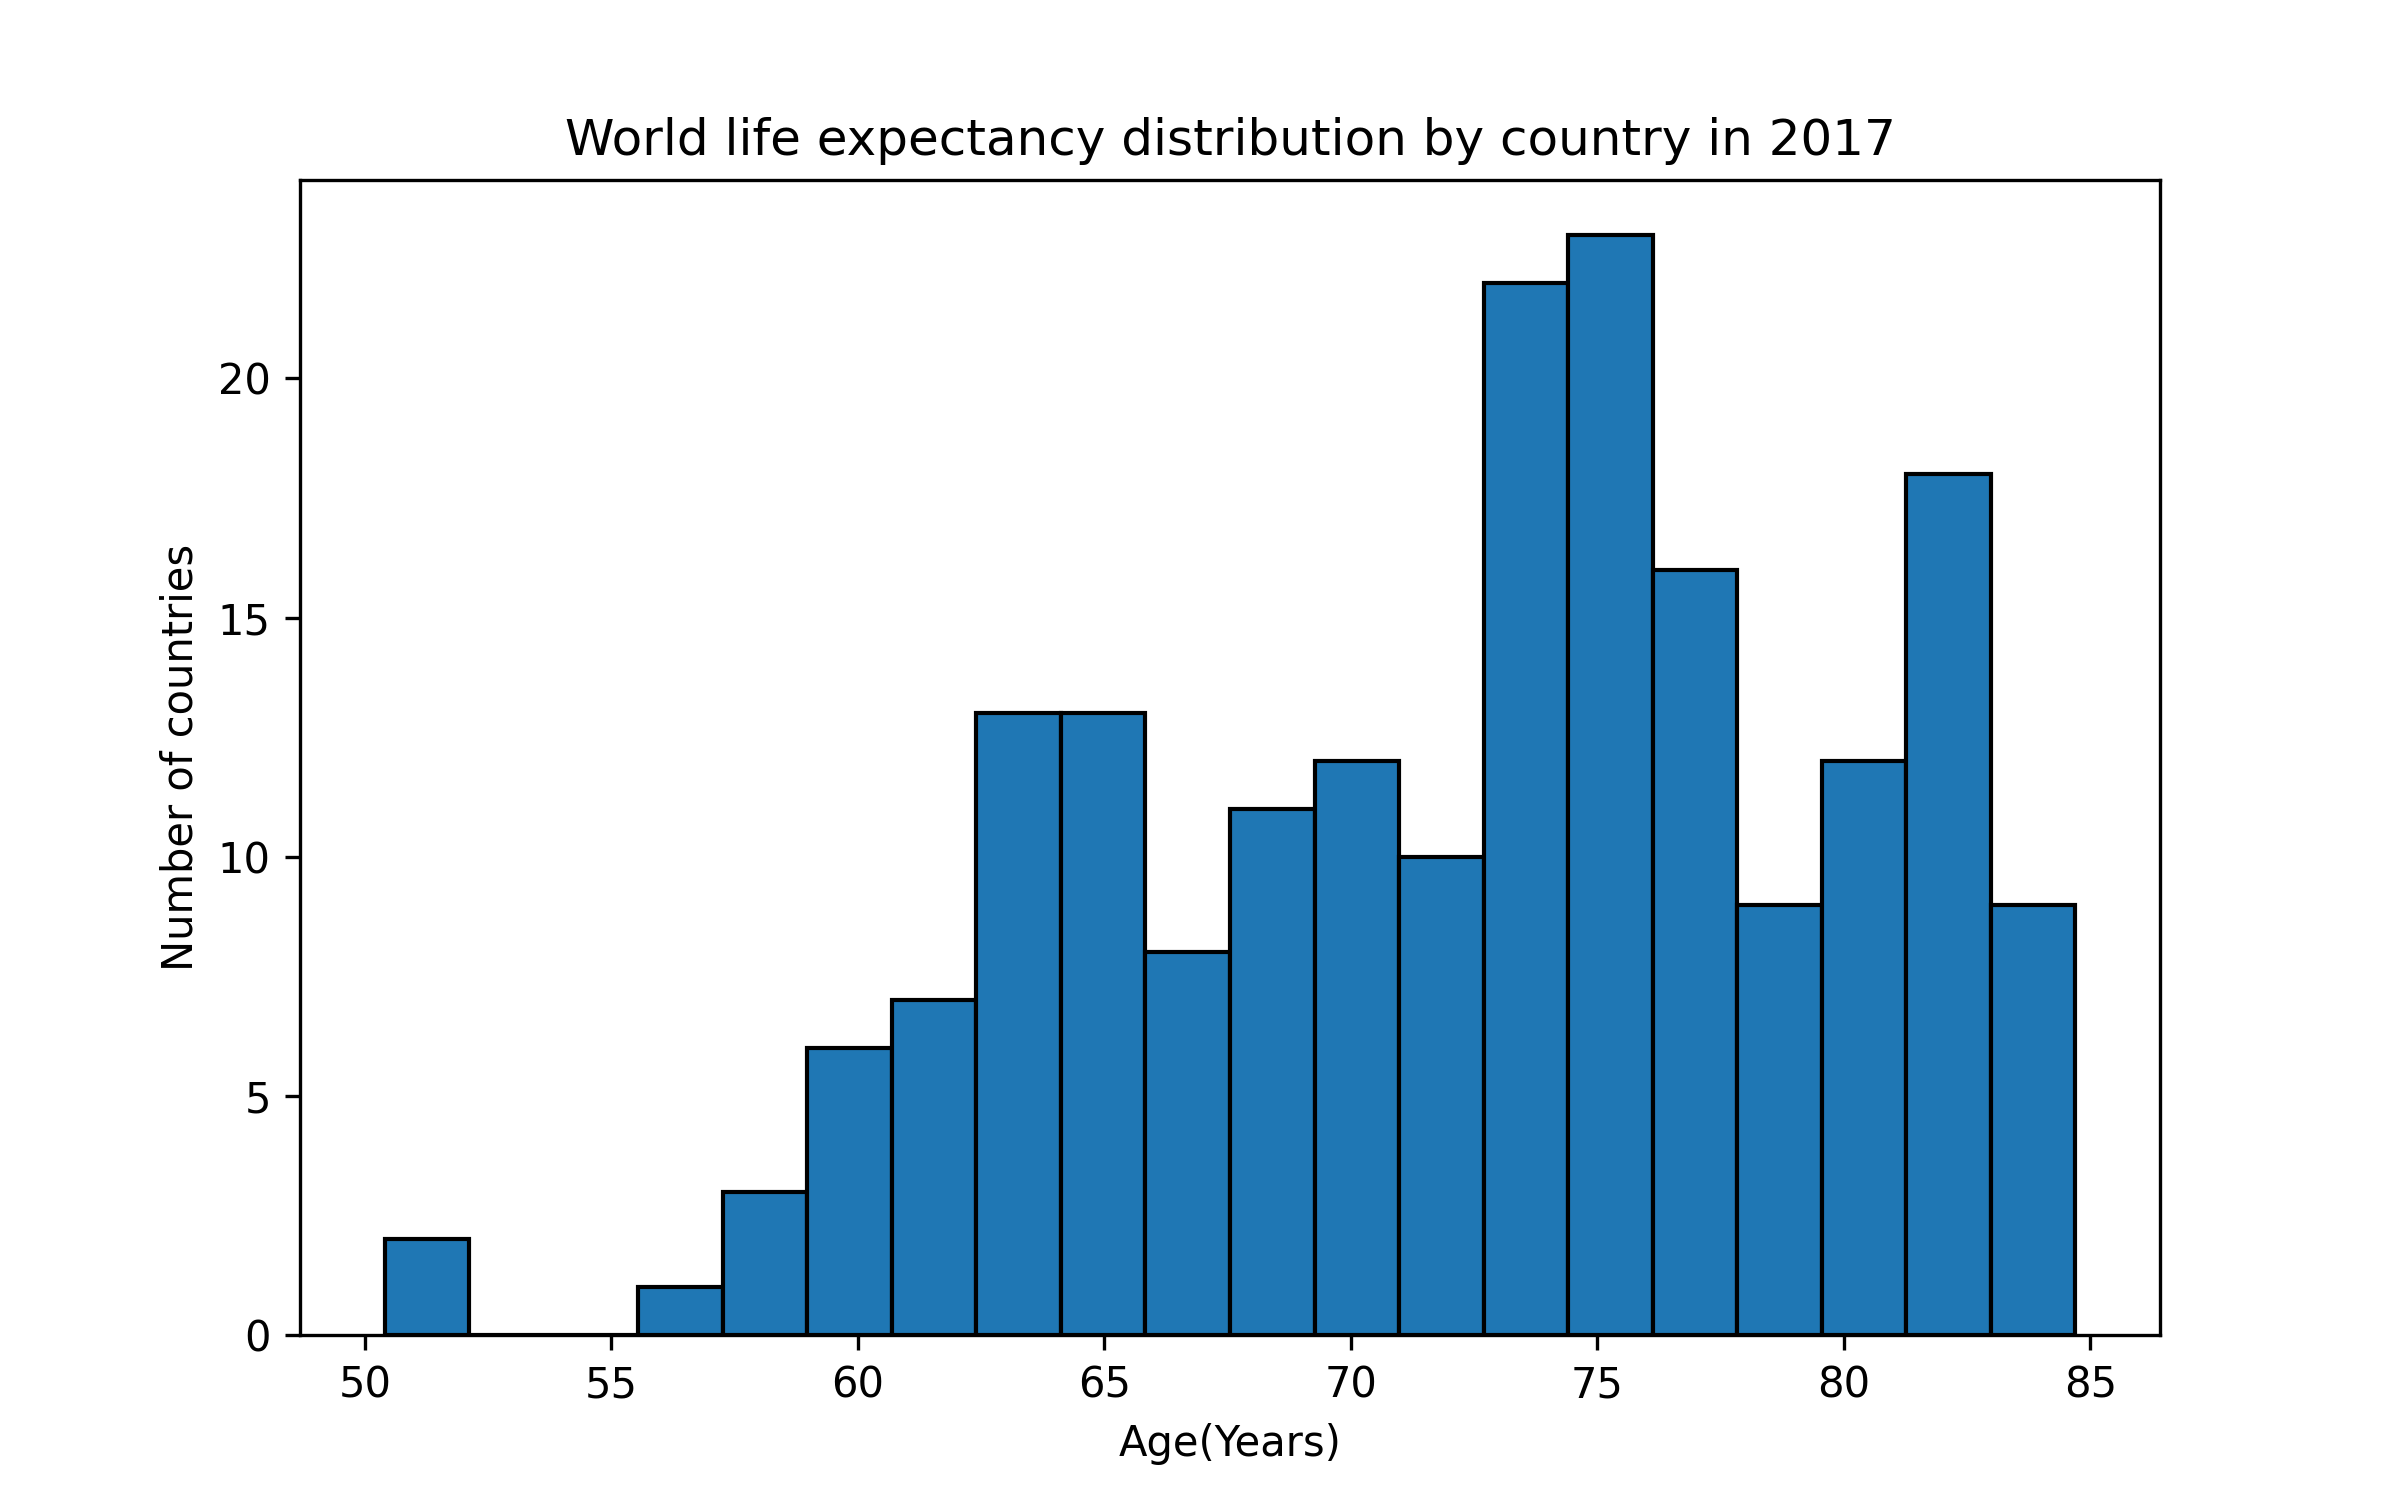
\includegraphics[width=0.8\textwidth]{figures/lex_histo.png}
    \caption{Distribution of Life expectancy in 2017}
    \label{fig:lex-dis}
\end{figure}
\section{Popultion's mean value confidence interval}
Given that our dataset comprises 195 observations, it is reasonable to presume a normal distribution with the preceeding estimations. 
The confidence interval can be calculated using this formula:
\begin{center}
    {\fontsize{16}{20}\selectfont $[\overline{x} - u_\beta \frac{s}{\sqrt{n}}, \overline{x} + u_\beta \frac{s}{\sqrt{n}}]$}
\end{center}
Nevertheless, when utilizing \href{https://scipy.org/}{SciPy}, it necessitates the specification of the "degree of freedom" parameter, which, in this instance, is determined as $195 - 1 = 194$.
The subsequent code illustrates the implementation of the formula for calculating the confidence interval of the mean values pertaining to GDP and Life Expectancy
\begin{verbatim}
    confidence_level = 0.95
    dof = size - 1
    alpha = (1 + confidence_level) / 2
    critical_value = scipy.stats.t.ppf(alpha, dof)
    print("c = ", critical_value)
    gdp_moe = critical_value * gdp_sd / np.sqrt(size)
    lex_moe = critical_value * lex_sd / np.sqrt(size)
    gdp_confidence_interval = (gdp_mean - gdp_moe, gdp_mean + gdp_moe)
    lex_confidence_interval = (lex_mean - lex_moe, lex_mean + lex_moe)
    print("GDP 95% confidence interval: ", gdp_confidence_interval)
    print("LEX 95% confidence interval: ", lex_confidence_interval)
\end{verbatim}
\newpage
Result:
\begin{verbatim}
    c =  1.972267532579456
    GDP 95% confidence interval:  (17457.119132515552, 24287.085995689573)
    LEX 95% confidence interval:  (71.36054581633697, 73.42817213238096)
\end{verbatim}